\documentclass{standalone}
\usepackage{tikz}
\usetikzlibrary{patterns, positioning}

\begin{document}
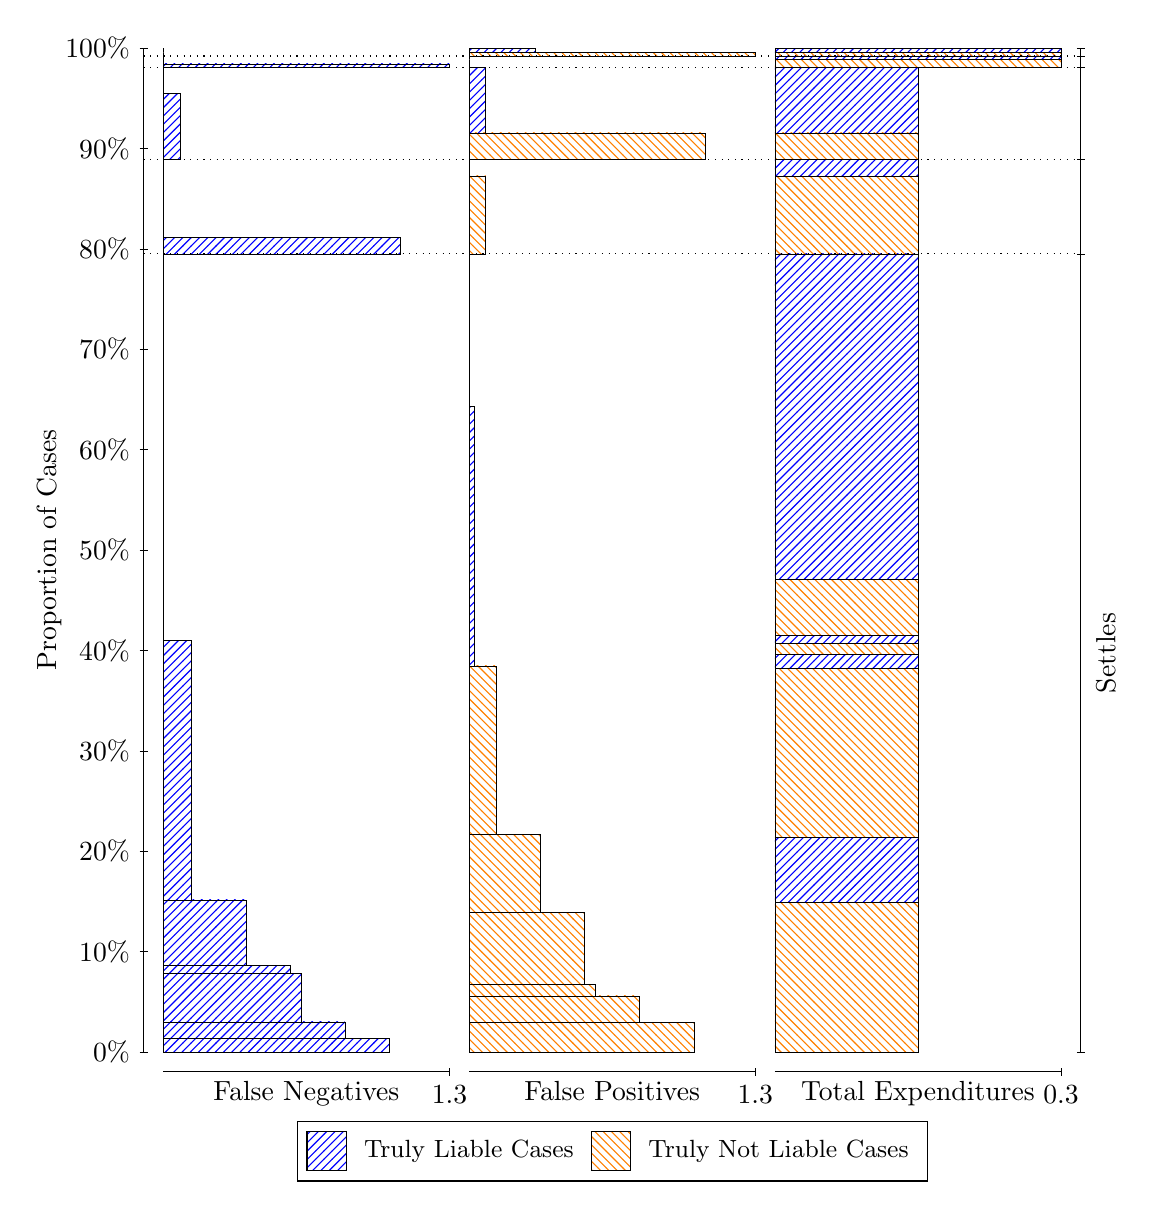
\begin{tikzpicture}
\draw[black, very thin] (1.5,1.75) -- (1.5,14.5);
\node[rotate=90, anchor=center] at (0.3, 8.125) {Proportion of Cases};
\draw[black, very thin] (1.45,1.75) -- (1.55,1.75);
\node[anchor=east] at (1.45, 1.75) {0\%};
\draw[black, very thin] (1.45,3.025) -- (1.55,3.025);
\node[anchor=east] at (1.45, 3.025) {10\%};
\draw[black, very thin] (1.45,4.3) -- (1.55,4.3);
\node[anchor=east] at (1.45, 4.3) {20\%};
\draw[black, very thin] (1.45,5.575) -- (1.55,5.575);
\node[anchor=east] at (1.45, 5.575) {30\%};
\draw[black, very thin] (1.45,6.85) -- (1.55,6.85);
\node[anchor=east] at (1.45, 6.85) {40\%};
\draw[black, very thin] (1.45,8.125) -- (1.55,8.125);
\node[anchor=east] at (1.45, 8.125) {50\%};
\draw[black, very thin] (1.45,9.4) -- (1.55,9.4);
\node[anchor=east] at (1.45, 9.4) {60\%};
\draw[black, very thin] (1.45,10.675) -- (1.55,10.675);
\node[anchor=east] at (1.45, 10.675) {70\%};
\draw[black, very thin] (1.45,11.95) -- (1.55,11.95);
\node[anchor=east] at (1.45, 11.95) {80\%};
\draw[black, very thin] (1.45,13.225) -- (1.55,13.225);
\node[anchor=east] at (1.45, 13.225) {90\%};
\draw[black, very thin] (1.45,14.5) -- (1.55,14.5);
\node[anchor=east] at (1.45, 14.5) {100\%};

\draw[black, very thin] (13.4,1.75) -- (13.4,14.5);
\draw[black, very thin] (13.35,1.75) -- (13.45,1.75);
\node[anchor=west] at (13.35, 1.75) {};
\draw[black, very thin] (13.35,11.885) -- (13.45,11.885);
\node[anchor=west] at (13.35, 11.885) {};
\draw[black, very thin] (13.35,13.083) -- (13.45,13.083);
\node[anchor=west] at (13.35, 13.083) {};
\draw[black, very thin] (13.35,14.256) -- (13.45,14.256);
\node[anchor=west] at (13.35, 14.256) {};
\draw[black, very thin] (13.35,14.399) -- (13.45,14.399);
\node[anchor=west] at (13.35, 14.399) {};
\draw[black, very thin] (13.35,14.5) -- (13.45,14.5);
\node[anchor=west] at (13.35, 14.5) {};

\draw[black, very thin, pattern color=blue, pattern=north east lines] (1.75,1.75) rectangle (4.6147,1.9256);
\draw[black, very thin, pattern color=blue, pattern=north east lines] (1.75,1.9256) rectangle (4.0558,2.1332);
\draw[black, very thin, pattern color=blue, pattern=north east lines] (1.75,2.1332) rectangle (3.4968,2.7458);
\draw[black, very thin, pattern color=blue, pattern=north east lines] (1.75,2.7458) rectangle (3.3571,2.8471);
\draw[black, very thin, pattern color=blue, pattern=north east lines] (1.75,2.8471) rectangle (2.7981,3.6824);
\draw[black, very thin, pattern color=blue, pattern=north east lines] (1.75,3.6824) rectangle (2.0994,6.9808);
\draw[black, very thin, pattern color=orange, pattern=north west lines] (1.75,6.9808) rectangle (1.75,11.885);
\draw[black, very thin, pattern color=blue, pattern=north east lines] (1.75,11.885) rectangle (4.7545,12.093);
\draw[black, very thin, pattern color=orange, pattern=north west lines] (1.75,12.093) rectangle (1.75,13.083);
\draw[black, very thin, pattern color=blue, pattern=north east lines] (1.75,13.083) rectangle (1.9596,13.919);
\draw[black, very thin, pattern color=orange, pattern=north west lines] (1.75,13.919) rectangle (1.75,14.256);
\draw[black, very thin, pattern color=blue, pattern=north east lines] (1.75,14.256) rectangle (5.3833,14.299);
\draw[black, very thin, pattern color=orange, pattern=north west lines] (1.75,14.299) rectangle (1.75,14.399);
\draw[black, very thin, pattern color=orange, pattern=north west lines] (1.75,14.399) rectangle (1.75,14.441);
\draw[black, very thin, pattern color=blue, pattern=north east lines] (1.75,14.441) rectangle (1.75,14.5);
\draw[black, very thin, pattern color=orange, pattern=north west lines] (5.6333,1.75) rectangle (8.4981,2.1253);
\draw[black, very thin, pattern color=orange, pattern=north west lines] (5.6333,2.1253) rectangle (7.7994,2.463);
\draw[black, very thin, pattern color=orange, pattern=north west lines] (5.6333,2.463) rectangle (7.2404,2.6054);
\draw[black, very thin, pattern color=orange, pattern=north west lines] (5.6333,2.6054) rectangle (7.1006,3.5194);
\draw[black, very thin, pattern color=orange, pattern=north west lines] (5.6333,3.5194) rectangle (6.5417,4.51);
\draw[black, very thin, pattern color=orange, pattern=north west lines] (5.6333,4.51) rectangle (5.9827,6.6544);
\draw[black, very thin, pattern color=blue, pattern=north east lines] (5.6333,6.6544) rectangle (5.7032,9.9528);
\draw[black, very thin, pattern color=blue, pattern=north east lines] (5.6333,9.9528) rectangle (5.6333,11.885);
\draw[black, very thin, pattern color=orange, pattern=north west lines] (5.6333,11.885) rectangle (5.8429,12.876);
\draw[black, very thin, pattern color=blue, pattern=north east lines] (5.6333,12.876) rectangle (5.6333,13.083);
\draw[black, very thin, pattern color=orange, pattern=north west lines] (5.6333,13.083) rectangle (8.6378,13.421);
\draw[black, very thin, pattern color=blue, pattern=north east lines] (5.6333,13.421) rectangle (5.8429,14.256);
\draw[black, very thin, pattern color=orange, pattern=north west lines] (5.6333,14.256) rectangle (5.6333,14.356);
\draw[black, very thin, pattern color=blue, pattern=north east lines] (5.6333,14.356) rectangle (5.6333,14.399);
\draw[black, very thin, pattern color=orange, pattern=north west lines] (5.6333,14.399) rectangle (9.2667,14.441);
\draw[black, very thin, pattern color=blue, pattern=north east lines] (5.6333,14.441) rectangle (6.4718,14.5);
\draw[black, very thin, pattern color=orange, pattern=north west lines] (9.5167,1.75) rectangle (11.333,3.6546);
\draw[black, very thin, pattern color=blue, pattern=north east lines] (9.5167,3.6546) rectangle (11.333,4.4748);
\draw[black, very thin, pattern color=orange, pattern=north west lines] (9.5167,4.4748) rectangle (11.333,6.6193);
\draw[black, very thin, pattern color=blue, pattern=north east lines] (9.5167,6.6193) rectangle (11.333,6.7949);
\draw[black, very thin, pattern color=orange, pattern=north west lines] (9.5167,6.7949) rectangle (11.333,6.9372);
\draw[black, very thin, pattern color=blue, pattern=north east lines] (9.5167,6.9372) rectangle (11.333,7.0385);
\draw[black, very thin, pattern color=orange, pattern=north west lines] (9.5167,7.0385) rectangle (11.333,7.7516);
\draw[black, very thin, pattern color=blue, pattern=north east lines] (9.5167,7.7516) rectangle (11.333,11.885);
\draw[black, very thin, pattern color=orange, pattern=north west lines] (9.5167,11.885) rectangle (11.333,12.876);
\draw[black, very thin, pattern color=blue, pattern=north east lines] (9.5167,12.876) rectangle (11.333,13.083);
\draw[black, very thin, pattern color=orange, pattern=north west lines] (9.5167,13.083) rectangle (11.333,13.421);
\draw[black, very thin, pattern color=blue, pattern=north east lines] (9.5167,13.421) rectangle (11.333,14.256);
\draw[black, very thin, pattern color=orange, pattern=north west lines] (9.5167,14.256) rectangle (13.15,14.356);
\draw[black, very thin, pattern color=blue, pattern=north east lines] (9.5167,14.356) rectangle (13.15,14.399);
\draw[black, very thin, pattern color=orange, pattern=north west lines] (9.5167,14.399) rectangle (13.15,14.441);
\draw[black, very thin, pattern color=blue, pattern=north east lines] (9.5167,14.441) rectangle (13.15,14.5);
\draw[black, dotted] (1.5,11.885) -- (13.4,11.885);
\draw[black, dotted] (1.5,13.083) -- (13.4,13.083);
\draw[black, dotted] (1.5,14.256) -- (13.4,14.256);
\draw[black, dotted] (1.5,14.399) -- (13.4,14.399);
\draw[black, very thin] (1.75,1.5) -- (5.3833,1.5);
\node[anchor=north] at (3.5667, 1.5) {False Negatives};
\draw[black, very thin] (5.3833,1.45) -- (5.3833,1.55);
\node[anchor=north] at (5.3833, 1.45) {1.3};

\draw[black, very thin] (5.6333,1.5) -- (9.2667,1.5);
\node[anchor=north] at (7.45, 1.5) {False Positives};
\draw[black, very thin] (9.2667,1.45) -- (9.2667,1.55);
\node[anchor=north] at (9.2667, 1.45) {1.3};

\draw[black, very thin] (9.5167,1.5) -- (13.15,1.5);
\node[anchor=north] at (11.333, 1.5) {Total Expenditures};
\draw[black, very thin] (13.15,1.45) -- (13.15,1.55);
\node[anchor=north] at (13.15, 1.45) {0.3};

\node[black, centered, rotate=90] at (13.72, 6.8176) {Settles};





\draw (7.449999999999999,1.5) node[draw=none] (baseCoordinate) {};
\begin{scope}[align=center]
        \matrix[scale=0.5, draw=black, below=0.5cm of baseCoordinate, nodes={draw}, column sep=0.1cm]{
            \node[rectangle, draw, minimum width=0.5cm, minimum height=0.5cm, pattern=north east lines, pattern color=blue] {}; &
            \node[draw=none, font=\small] (B) {Truly Liable Cases}; &
            \node[rectangle, draw, minimum width=0.5cm, minimum height=0.5cm, pattern=north west lines, pattern color=orange] {}; &
            \node[draw=none, font=\small] (B) {Truly Not Liable Cases}; \\
            };
\end{scope}

\end{tikzpicture}
\end{document}